\chapter{Introduction}

\section{Adaptive Vehicle Make (AVM) Overview}
The AVM program has developed tools (referred to as META tools)for designing Cyber Physical (or Mechatronic) Systems. Exemplified by modern Amphibious and Ground Military Vehicles, these systems are increasingly complex, take much longer to design and build, and are increasingly costlier. The vision of the AVM program is to revolutionize the design methodology of such systems and reduce the design time to 1/5th of the traditional systems engineering V methodology (MIL–STD-499). 

The META tools realize this vision by advancing a novel design flow geared around the following core concepts:

\begin{itemize}
\item \textbf{Component-Based Design} enables design cycle compression by reuse of existing technology and knowledge, encapsulated in integratable and customizable components that can be rapidly used in a design. Components in CPS are heterogeneous, span multiple domains (physical – thermal, mechanical, electrical, fluid , .. and computational – software,  computing platforms), and require multiple models to soundly represent the behavior, geometry, and interfaces, at multiple levels of abstractions. 
 
\item \textbf{Design Space Exploration} using explicit representation of design choices and parameterized components. META tools enable a designer to systematically engineer a flexible and comprehensive design space for sub-systems and system that can be explored for satisfying requirements. The design spaces for subsystems and systems are assets that encapsulate design knowledge, which can be reused in a context different from which it was originally created. \textit{Multi-Scale Design Space Exploration} incorporates multiple analysis methods that trade accuracy with computation time for exploring the large design spaces, and iteratively converge over to design points of interest.

\item \textbf{Testbenches for Design Evaluation} capture requirements in a form that can be automatically evaluated for a system-under-test, using a large set of domain-specific analyses – ranging from hybrid dynamics simulation, software platform timing simulation, geometric parameter evaluation, finite element analysis, probabilistic certificates of correctness, among others. The model composition tools included in META operate over defined testbenches and synthesize artifacts necessary for executing analysis in pertinent domain tools such as Dymola, Pro-e/Creo, Truetime, Qualitative Envisionment, Abaqus, etc.. 
\end{itemize}

% Replace with a different design flow figure
\begin{figure}
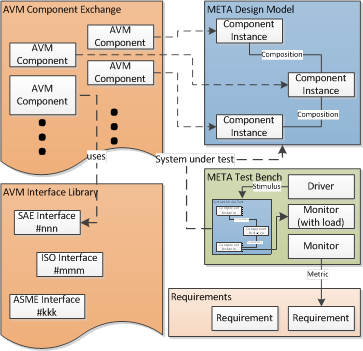
\includegraphics{DesignFlow}
\caption{AVM Design Flow}
\label{Intro_DesignFlow}
\end{figure}

\section{AVM Component Overview}
A central idea in engineering is that complex systems are built by assembling less complex components (building blocks). One approach, Component-based design offers advantages with respect to monolithic design such as reuse of design solutions, modular analysis and validation, reconfigurability and complexity management. In the context of component-based design the concept of component is much richer than the concept of containment. As opposed to monolithic design synthesis, it enables the formulation of the design problem the following manner: \textit{“design a system meeting the requirements using a set of components”}, where requirements specify essential properties of the system.

Component-based design requires a composition framework that satisfies two requirements:
\begin{itemize}
\item \textit{Composability}: meaning that components do not change their essential properties after composed with other components.
\item \textit{Compositionality}: meaning that the essential properties of the system can be computed from the properties of its components.
\end{itemize}
Composition frameworks enable constructivity: the synthesis of systems with predictable properties from components with known properties.

Within this context, AVM components are heterogeneous cyber-physical system components, spanning exclusively cyber, exclusively physical, as well as cyber-physical. Meaningful AVM components capture non-trivial and re-usable design knowledge, have interfaces for composition, and represent the design knowledge in a formalism that enables automated composition. AVM Components in general, could be composed of many parts and subparts; however, for the purposes of the AVM program and this document, AVM components are considered as atomic (black-box) units that can be acquired off-the shelf or custom built, and can be composed together into a system. 

An AVM Component model is an integrated multi-model including an integration model (a model wrapper) that represents the key properties, parameters, compositional interfaces and their association with domain models; and a number of domain models that represent the dynamics, geometry, computational (cyber), and manufacturing of the component at multiple levels of abstraction and fidelity. 


\begin{figure}
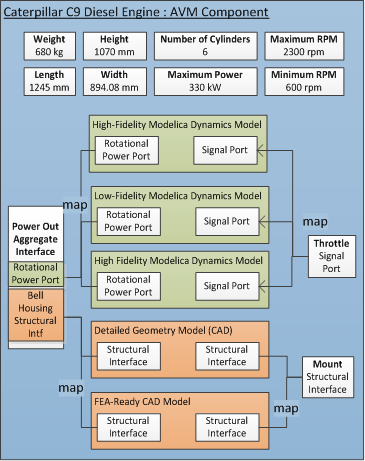
\includegraphics{ComponentConcept}
\caption{AVM Component Model Conceptualization}
\label{Intro_Component}
\end{figure}

The figure \ref{Intro_Component} illustrates an AVM component model consisting of a set of properties (e.g. Weight, Height, Maximum Power, etc.), a set of parameters (properties that are user modifiable), a set of interfaces – which can be atomic (e.g. Throttle Signal Port) as well as aggregate (e.g. Power Out Aggregate Interface consisting of a Rotational Power Port, and a Bell Housing Structural Port), a set of embedded domain models (e.g. High-Fidelity Modelica Dynamics Model, FEA-Ready CAD Model, etc.) representing different fidelities and abstraction of the component dynamics and geometry. The domain models are developed and represented in external tools and languages (i.e. Modelica/Dymola, CAD/Pro-E). The integration model contains references to the domain models (through a URI) and explicitly represents domain-model specific interfaces (e.g. Rotational Power Port, Structural Interface, etc.) that are mapped into the external interfaces of the Component.

\section{Scope}
The scope of this document is limited to the specification of AVM Component Model. The AVM Design Models that are composed together using AVM Components, and the META Language, Tools, and Design Flow are considered outside the scope of this document. The domain modeling tools (such as Dymola, Pro/E, ...)and languages (Modelica, CAD, ) are outside the scope of this document, however, modeling guidelines that must be adhered to when creating domain models are included in this document.

\section{Purpose}
The purpose of this document is to serve as a reference guide for AVM component developers enabling them to rapidly author valid components that can be used within the META Tools. The document purports to define and explain AVM Component Models, with specific emphasis on the integration model, and introduce methods to author and validate AVM Component models.


\section{Document Organization}
The rest of this document is organized as follows. 
\begin{enumerate}
\item Chapter 1 provides a very brief overview of the AVM tools and rationale for the AVM component model
\item Chapter 2 provides a detailed description of the syntax and semantics of the AVM Component Model and its constituent parts
\item Chapter 3 describes a framework for authoring AVM Components
\item Chapter 4 describes a validation suite and automated testing framework for validating component designs
\end{enumerate}